\documentclass[a4paper]{article} %%% use \documentstyle for old LaTeX compilers

\usepackage[portuguese]{babel} %%% 'french', 'german', 'spanish', 'danish', etc.
\usepackage{makeidx}
\usepackage{multirow}
\usepackage{multicol}
\usepackage[dvipsnames,svgnames,table]{xcolor}
\usepackage[dvips]{graphicx} 
\usepackage[utf8x]{inputenc}
\usepackage{epstopdf}
\usepackage{ulem}
\usepackage{hyperref}
\usepackage{amsmath}
\usepackage{amssymb}
\usepackage{txfonts}
\usepackage{mathdots}
\usepackage[classicReIm]{kpfonts}

% You can include more LaTeX packages here 

\usepackage[a4paper,top=2.5cm,bottom=2.5cm,left=3cm,right=3cm,marginparwidth=1.75cm]{geometry}
\begin{document}

%\selectlanguage{english} %%% remove comment delimiter ('%') and select language if required

\title{Movimento planetário}
\author{Bruno da silva}

\fontfamily{phv}\selectfont
\begin{titlepage}
	\begin{center}
		{\scshape\Large Universidade Federal Fluminense -UFF \par}
		\vspace{7cm}
		{\huge\bfseries Movimento planetário \par}
		\vspace{5.5cm}
		{\itshape Autor Bruno da Silva Machado \par}      
		
		\vspace{6.5cm}    
		
		\vfill
		{\large \today\par}
	\end{center}
\end{titlepage}
\setcounter{secnumdepth}{0}

\section{Introdu\c{c}\~{a}o}

\noindent

O movimento planet\'{a}rio \'{e} aquele os planeta fazem ao redor de uma estrela este movimento obedecem as leis de Kepler, que por sua v\^{e}z podem ser obtidas pelas leis de Newton

Neste trabalho vamos estudar melhor este tipo de movimento analisar algumas de suas caracter\'{i}sticas atrav\'{e}s de m\'{e}todo num\'{e}rico.

Usaremos o m\'{e}todo de Verlet por sua simplicidade e estabilidade por nos fornece uma boa aproxima\c{c}\~{a}o num\'{e}rica para o problema em questão.

\noindent 
\section{Estudo do Movimento Planet\'{a}rio}

\noindent 

Considere um planeta girando em torno de uma estrela e a for\c{c}a entre esses corpos \'e a gravidade. De acordo com a lei de gravita\c{c}\~{a}o universal de Newton podemos descrever a for\c{c}a de intera\c{c}\~{a}o entre os corpos como:
\[F_G = \frac{GM_sM_E}{r^{2}}\]

Onde $\ M_s$ e $\ M_E$ s\~{a}o a massa do Sol e da Terra por exemplo,$\ r$ e a distancia entre eles, e $\ G$ \'{e} constante gravitacional. Agora vamos assumir a massa do sol \'{e} suficientemente grande de modo que seu movimento possa ser desprezado. Nos fazemos isto para calcular a posição do planeta em fun\c{c}\^{a}o do tempo. Aplicando a segunda lei de Newton do movimento temos: 
\[\overrightarrow{F} = m\overrightarrow{a}\]
\[F(x,y) = m\left(\frac{d^{2}x}{dt^2}\textbf{i} + \frac{d^{2}y}{dt^2}\textbf{j}\right)\]
Fazendo $\ y = 0 $ ou $\ x = 0$ na equa\c{c}\~{a}o anterior temos que:
\[\frac{d^2x}{dt^2} = \frac{F_x}{m}\]
\[\frac{d^2y}{dt^2} = \frac{F_y}{m}\]
Onde $\ F_x$ e $\ F_y$ s\~{a}o componentes da for\c{c}a gravitacional e dessa forma podemos reescreve-los como:
\begin{equation}
F_x = -\frac{GM_EM_E|x|}{x^3}\textbf{i}
\end{equation}
e 
\begin{equation}
F_y = - \frac{GM_EM_E|y|}{y^3}\textbf{j}
\end{equation}
Onde o sinal negativo de $\ F_x$ indica que a for\c{c}a esta direcionada para o Sol,quando este est\'{a} localizado na origem do sistema de coordenadas.

\begin{center}
	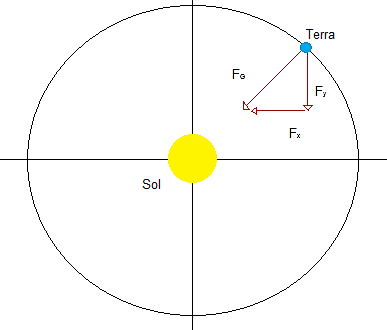
\includegraphics[width=3.87in, height=3.50in, keepaspectratio=false]{image1.png}
	
	\scriptsize{ Figura1. sistema de coordenadas para descrever o movimento da terra em relação ao Sol. O Sol esta na origem do sistema. A força gravitacional $F_g$ exerce força que mantem o planeta orbitando é um agente responsável pelo período da terra. }
\end{center}

Agora vamos a abordagem usual de escrever as equações diferenciais de segunda ordem em equação de primeira ordem.

\[\frac{d^2x}{dt^2} = \frac{d}{dt}\left(\frac{dx}{dt}\right) \]
\[\frac{d^2y}{dt^2} = \frac{d}{dt}\left(\frac{dy}{dt}\right) \]
dessa forma temos:
\[\frac{dx}{dt} = v_x\] 
\[\frac{dv_x}{dt} = -\frac{GM_Sx}{r^3}\]

\[\frac{dy}{dt} = v_y\] 
\[\frac{dv_y}{dt} = -\frac{GM_Sy}{r^3}\]

Estes podem ser convertidos em equações diferencias que podem ser solucionado numericamente. no entanto, antes de proceder com isso, \'{e} útil para considerar a escolha de unidades. Uma opção é simplesmente usar unidades SI não há nenhuma dificuldade em usa-las, exceto que metros e segundos não correspondem a escala do problema por exemplo, o raio da órbita terrestre de é aproximadamente igual a $\ 1.5 x10^{11}$ m. Se usarmos as unidades SI, um gr\'{a}fico que mostra a \'{o}rbita em torno do Sol teria r\'{o}tulos de $\ 1x10^11, 2x10^11 m$, etc. Isso seria estranho, embora n\~{a}o incrivelmente assim. \'{e} muito mais conveniente para usar as unidades astron\^{o}micas, AU, que s\~{a}o definidas a seguir. uma unidade astron\^{o}mica de comprimento equivale a dist\^{a}ncia media entre o sol e da terra que \'{e} aproximadamente $\ 1.5 X 1^11 m$. \'{e} conveniente para medir o tempo em anos ($\ 1 ano \approx 3,2 X 10^7 S$) uma vez que esta unidade coincide com o sistema solar melhor do que, por exemplo, segundos. Vamos, portanto, usar unidades astron\^{o}micas de dist\^{a}ncia, e medir tempo em anos, a menos que seja indicado e para completar o nosso sistema de unidades tamb\'{e}m precisamos uma correspond\'{e}ncia em unidade de massa. Este \'{e} facilmente obtido se lembrarmos que a \'{o}rbita da terra de é aproximadamente, circular. para movimento circular n\'{o}s sabemos que a força deve ser igual a $\ M_Ev^2/r$, o que nos leva a:

\[F_G = \frac{M_Ev^2}{r} = \frac{GM_SM_E}{r^2}\]
onde V \'{e} a velocidade da terra.

\[M_Ev^2r = GM_SM_E\]
\[GM_S = v^2r \]

lembrando que $\ v = \frac{2\pi}{r}$ e $\ r = 1AU$ temos ent\~{a}o $\ GM = 4\pi^2 AU^3/yr^2$

\section{Resultados}

A partir das relações anteriores podemos chegar nas solu\c{c}\~{o}es num\'{e}ricas 

\[a_{x,t} = -\frac{4\pi^2x_t}{r_t^3}\]
\[x_{t+1} = x_t +v_{x,t+1}\Delta{t} + 1/2a_{x,t}\Delta{t} \]
\[v_{x,t+1} = v_{x,t} + a_{x,t}\] 
\[a_{y,t} = -\frac{4\pi^2y_t}{r_t^3}\]
\[y_{t+1} = y_t +v_{y,t+1}\Delta{t} + 1/2a_{y,t}\Delta{t} \]
\[v_{y,t+1} = v_{y,t} + a_{y,t}\] 

Para avaliar o que obtemos vamos exemplifica-lo seja $\Delta{t}$ o passo temporal bem pequeno valendo 0.0001 ano e y a distancia no eixo das ordenadas valendo 1AU e x = 0 a velocidade no eixo é vy = 2$\pi$ AU/ano e no eixo das abcissas vx = 0.

\begin{center}
	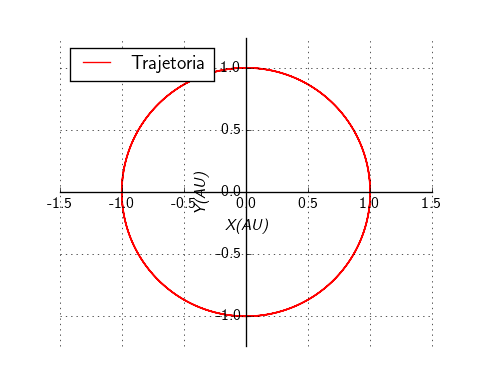
\includegraphics[width=4.80in,height=3.84in, keepaspectratio=false]{image1_15-50-59-772000.png}
	
	\scriptsize{Figura2. terra orbitando o Sol.}
\end{center}

Como podemos ver acima a orbita da terra \'{e} uma circunfer\^{e}ncia de raio 1 AU, mas sabemos que das leis de Kepler que as orbitas dos planetas descrevem uma elipse com o sol em um dos seus focos,porem como a orbita terrestre e bem pr\'{o}xima de uma circulo (i.e.,sua excentricidade e de apenas 0.017 que \'{e} um valor bem pequeno) nosso exemplo se aproxima de maneira eficiente com a realidade

Aumentando um pouco a velocidade inicial acrescentando 0.1, 0.5 e 1 a $v_y = 2\pi$, temos uma mudança na trajetória ela começa a se tornar elíptica uma vez sua energia varia entre $V_{min} < E < 0$, podemos ver isso nas figuras a seguir 

\vspace{1.1cm}

\begin{center}
	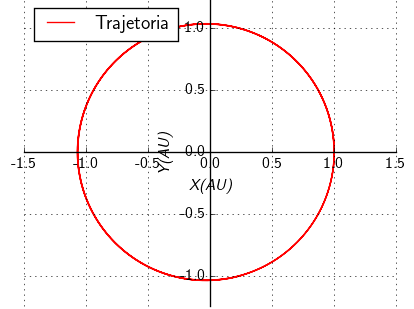
\includegraphics[width=4.14in,height=3.09in, keepaspectratio=false]{image2_15-50-59-794000.png}
	
	\scriptsize {Figura 3.Para um acréscimo de 0.1, a trajetória não sofre uma mudança drástica ao ponto de podermos notar algum tipo de diferença significativa Mas é possível notar que o deslocamento da partícula se estendeu para o lado esquerdo.}
	
\end{center}

\vspace{1.1cm}

\begin{center}
	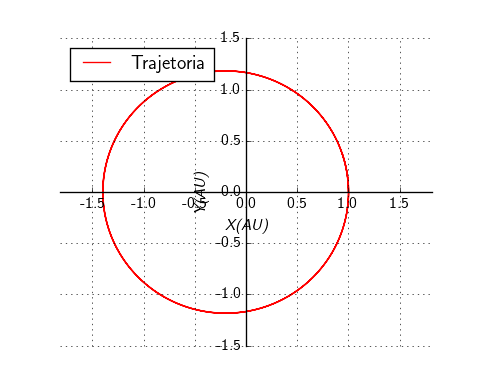
\includegraphics[width=3.98in,height=3.44in, keepaspectratio=false]{image3_15-50-59-818000.png}

	
	\scriptsize {Figura 4.Agora, para um acréscimo de 0.5, está mais nítido o que foi citado na figura anterior. A trajetória se estende para a esquerda e o raio da "circunferência" aumenta.}
	
\end{center}



\begin{center}
	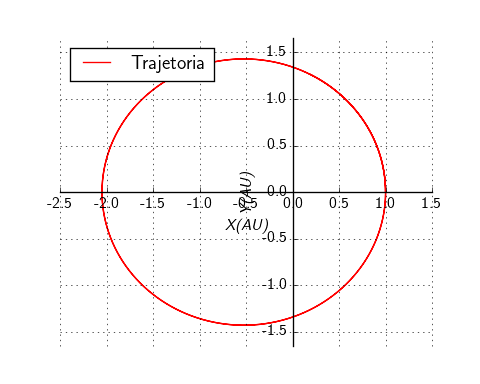
\includegraphics[width=4.80in,height=3.84in, keepaspectratio=false]{image4_15-50-59-718000.png}
	
	\scriptsize{Figura 5.Para um acréscimo de 1 a velocidade inicial, nota-se que a trajetória prossegue se estendendo para a esquerda e é acrescentado para ambos sentidos do eixo y.}
	
\end{center}

Notemos que quando a velocidade é acrescentada de algum valor a trajetória aumenta e se estende para a esquerda. A velocidade acrescentada foi em $v_y$ e o começo da trajetória do planeta está em $X=1$ e $Y=0$. Então segue -se subindo com uma velocidade um pouco maior, e da 2ª Lei de Kepler, a área percorrida pela Terra em um período de tempo igual deve ser a mesma. Logo como a Terra tem velocidade maior na parte positiva do eixo x, quando ela estiver fazendo a trajetória na outra extremidade da elipse ela deve ter velocidade menor, pois deve percorrer a mesma área.

porem exite um limite em que podemos aumentar a velocidade e manter a orbita fechada. Supondo que ha conservação de energia temos que a energia total e fornecida pela equação abaixo:

\begin{equation}
	E = \frac{1}{2}mv^2 - \frac{GMm}{r}
\end{equation} 
onde v e x são o modulo da velocidade e posição respectivamente.

como dito anteriormente para a orbita ser fechada $V_{min}< E < 0$ substituindo em (4) temos a seguinte inequação

\[\frac{1}{2}mv^2 - \frac{GMm}{r} < 0\]
\[\frac{1}{2}mv^2 < \frac{GMm}{r}\]
\[mv^2 < \frac{2GMm}{r}\]
\[v^2 < \frac{2GM}{r}\]
\begin{equation}
	v < \sqrt{\frac{2GM}{r}}
\end{equation}

A solução acima e familiar ela é a equação da velocidade de escape, ou seja, para que a orbita seja fechada a velocidade do satélite de ser menor que a de escape.

\subsection{Espaço de fase em x para velocidades diferentes}
\noindent

Vamos analisar agora o espaço de fase (em x) para cada caso de velocidade diferente já apresentado. Na Figura 6 novamente não há uma mudança significativa para algum tipo de análise, mas podemos notar que o movimento conserva energia e que a velocidade matem a transição para x positivo e negativo. A Figura 7 apresenta algumas características diferentes em relação a primeira, mas vamos analisar melhor utilizando a Figura 8, pois ela é a que deixa mais nítido o que ocorre quando a velocidade é aumentada, os trechos em que ela se mantem são os ápices, ou seja, quando $x = \pm1$ e $y = \pm1$, ou seja, a velocidade máxima e mínima continuam as mesmas, mas a transição entre elas é diferente. Note no gráfico da Figura 6 que a quando $x < 0$ a transição é mais longa que quando $x > 0$.
\begin{center}
	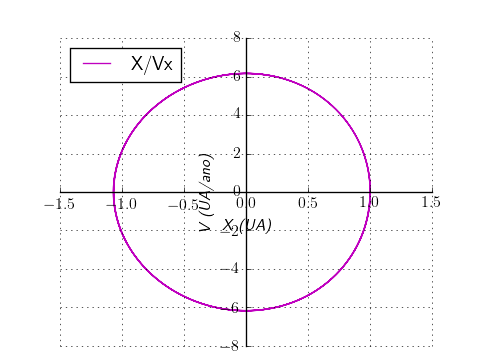
\includegraphics[width=4.80in,height=3.56in, keepaspectratio=false]{image2_15-51-19-589000.png}
	
	\scriptsize {Figura 6. Gráfico com pouca informação sobre a alteração da velocidade.}
\end{center}

\begin{center}
	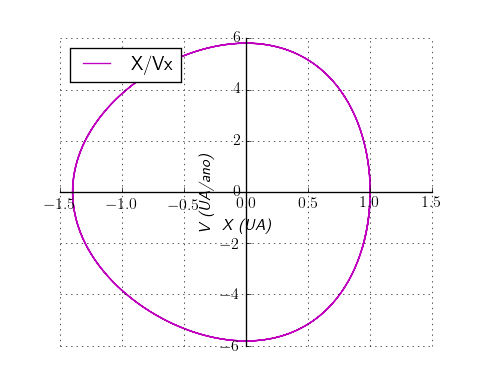
\includegraphics[width=4.80in,height=3.84in, keepaspectratio=false]{image3_15-51-12-345000.png}
	
	\scriptsize {Figura 7. Gráfico com ligeira mudança para $x<0$.}
\end{center}

\begin{center}
	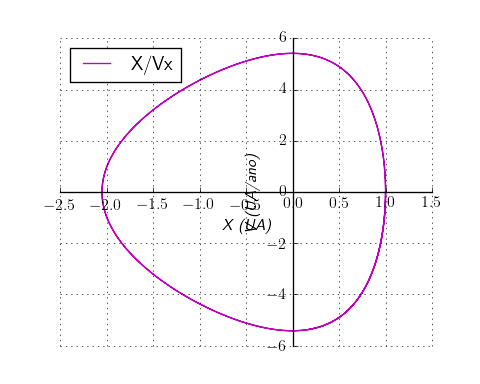
\includegraphics[width=4.80in,height=3.84in, keepaspectratio=false]{image4_15-51-08-565000.png}
	
	\scriptsize {Figura 8. Gráfico com melhor informação sobre as consequências de mudar a velocidade inicial do movimento.}
\end{center}

\subsection{Espaço de fase para velocidades diferentes}

Agora, nas figuras a seguir temos o espaço de fase do 'raio' (distância do centro da circunferência até a Terra) em relação ao módulo da velocidade. 

\begin{center}
	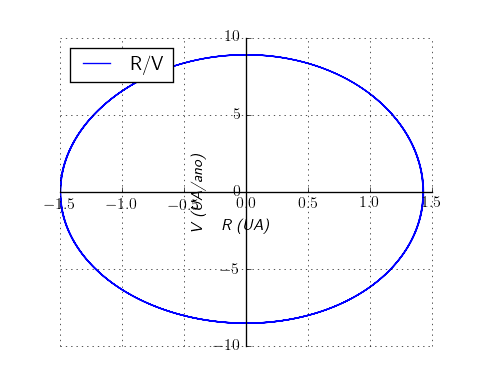
\includegraphics[width=4.80in,height=3.84in, keepaspectratio=false]{image2_15-51-24-116000.png}
	
	\scriptsize {Figura 9. Neste gráfico o raio sofre um pequeno aumento quando a velocidade.}
\end{center}

\begin{center}
	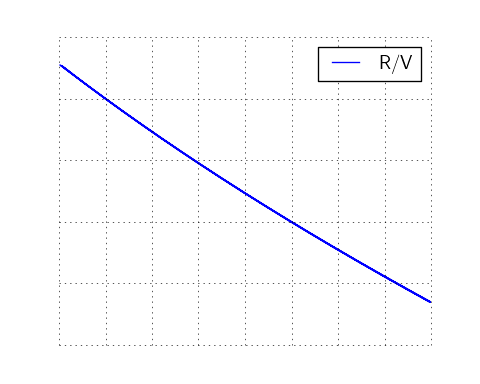
\includegraphics[width=4.80in,height=3.84in, keepaspectratio=false]{image3_15-51-18-639000.png}
	
	\scriptsize {Figura 10. Gráfico com um aumento um pouco maior da velocidade inicial, pode-se notar um aumento considerável de $v$ conforme $r$ aumenta.}
\end{center}

\begin{center}
	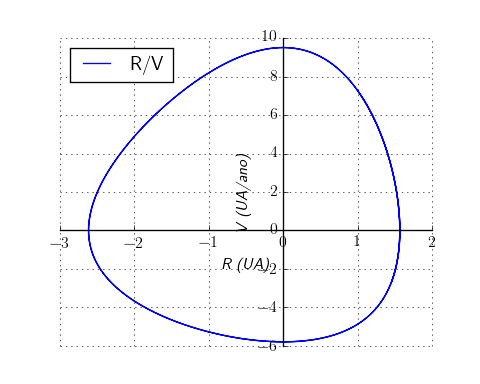
\includegraphics[width=4.80in,height=3.85in, keepaspectratio=false]{image4_15-51-15-338000.png}
	
	\scriptsize {Figura 11. Neste gráfico o aumento significativo de até um AU, a velocidade diminui drasticamente.}
\end{center}

\subsection{Excentricidade da órbita}

A excentricidade da órbita é dada por 

\begin{equation}
e = \sqrt{1 - \frac{b^2}{a^2}}, \qquad \forall (b\leq a)
\end{equation}

Usando o método de Verlet e fazendo um gráfico da excentricidade pelo acréscimo da velocidade inicial (Figura 11), nota-se que a excentricidade tende para 1, ou seja, o movimento representa uma elipse com a diferença dos raios $a$ e $b$ aumentando e acaba por representar uma parábola($e=1$).
\begin{center}
	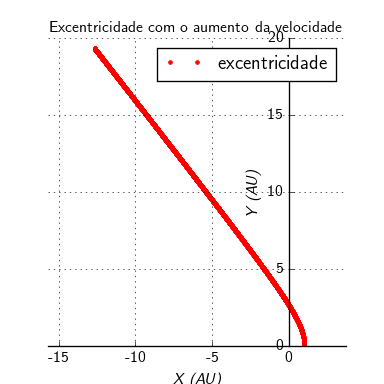
\includegraphics[width=3.84in,height=3.84in]{excentricidade.png}
\end{center}


\section{Conclus\~{a}o}

Conclu\'{i}mos que para orbitas circulares e elípticas as equações acima nos fornecem uma boa aproximação em relação comas orbitas planetárias reais, também e possível, através de ajustes, deduzimos e verificar a veracidade da 3$^\circ$ lei de kepler e que a relação entre o período e o raio da orbita dos planetas corre de forma logarítmica, e que as leis de Kepler e algo bem mais geral podendo descrever e prever o movimento de satélites e as leis de Newton são bem sucedidas em abordar as leis de Kepler de forma analítica são peça fundamental para a analise numérica feita neste trabalho



\section{Bibliografia}

\noindent 

\indent Bruno da Silva Machado, Leis de Kepler, 2017

\indent N. J. Giordano \& H. Nakanishi, Computational Physics, 2${}^\circ$ed, 2007

\indent  M\'etodo de Verlet, Wikip\'edia a enciclop\'edia livre, 2017

\indent Sears \& Zemansky, F\'{i}sica 2 Termodin\^{a}mica e ondas, 12${}^\circ$ed, 2008

\indent Talita A.Anjos, Brasil Escola,2016


\end{document}

